\subsubsection{bringit::client::bringit::Bringit}

\label{bringit::client::bringit::Bringit}
\begin{figure}[H]
	\centering
	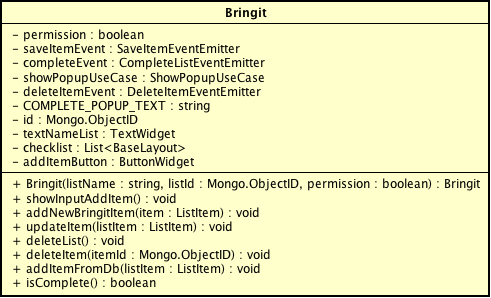
\includegraphics[scale=0.5]{Sezioni/SottosezioniST/img/app/Bringit.png}
	\caption{bringit::client::bringit::Bringit}
\end{figure}

\begin{itemize}
\item \textbf{Descrizione}: Classe che contiene la vera e propria bolla lista-spesa dell'applicazione. Estende Basebubble e utilizza i servizi forniti dall'SDK Monolith.
\item \textbf{Utilizzo}: La classe è il cuore dell'applicazione, conterrà i vari prodotti della lista e potrà essere inoltrata o pubblicata ai vari utenti.
\item \textbf{Attributi}: 
	\begin{itemize}
	\item \textit{private permission:boolean}\\
	L'attributo relativo ai permessi della specifica lista bringit.
	\item \textit{private saveItemEvent:SaveItemEventEmitter}\\
	L'oggetto relativo all'emissione degli eventi relativi al salvataggio dei prodotti della lsita.
	\item \textit{private completeEvent:CompleteEventEmitter}\\
	L'oggetto relativo all'emissione degli eventi relativi al completamento della lsita.
	\item \textit{private deleteItemEvent:DeleteItemEventEmitter}\\
	L'oggetto relativo all'emissione degli eventi relativi all'eliminazione dei prodotti della lsita.
	\item \textit{private id:string}\\
	L'identificativo della lista bringit.
	\item \textit{private COMPLETE\_POPUP\_TEXT:string}\\
	Il messaggio che viene visualizzato una volta completata la lista bringit.
	\item \textit{private textNameList:TextWidget}\\
	Il widget di testo contenente il nome della lista.
	\item \textit{private checklist:ChecklistItemWidget[]}\\
	L'array contenente i widget di check associati ai prodotti.
	\item \textit{private addItemButton:ButtonWidget}\\
	Il bottone che permette l'aggiunta di un nuovo prodotto alla lista.
	\item \textit{private showPopupUseCase:ShowPopupUseCase}\\
	\end{itemize}
\item \textbf{Metodi}:
	\begin{itemize}
	\item \textit{public Bringit(listName:string,listId:string,permission:boolean):Bringit}\\
	Il costruttore della classe bringit.
					\\ \textbf{Parametri}: \begin{itemize}
			\item \textit{listName:string}\\
			Il nome della lista bringit.
			\item \textit{listId:string}\\
			L'identificativo della lista bringit. Se è vuoto verrà creato al momento dal costruttore.
			\item \textit{permission:boolean}\\
			L'attributo relativo ai permessi della specifica lista bringit. Se è a true significa che l'utente che visualizza la lista ha i permessi, e verrà aggiunto alla lista il bottone che rende possibile l'aggiunta di nuovi prodotti alla lista.
					\end{itemize}
	\item \textit{public deleteList():void}\\
	Elimina la lista da tutte le chat e dal database.
	\item \textit{public showInputAddItem():void}\\
	Questo metodo mostra la form di input per l'aggiunta dei dati relativi a un nuovo prodotto da aggiungere alla lista bringit.
	\item \textit{public isComplete():boolean}\\
	Questo metodo ritorna true se la lista è completata, false altrimenti.
	\item \textit{public addItemFromDb(listItem:ListItem):void}\\
	Aggiunge un prodotto alla lista, prendendolo dal database.
				\\ \textbf{Parametri}: \begin{itemize}
			\item \textit{listItem:ListItem}\\
			Il prodotto da aggiungere alla lista.
					\end{itemize} 
	\item \textit{public deleteItem(itemId:string):void}\\
	Elimina uno specifico item da tutte le chat e dal database.
				\\ \textbf{Parametri}: \begin{itemize}
			\item \textit{itemId:string}\\
			L'identificativo del prodotto da eliminare.
					\end{itemize}
	\item \textit{public addNewBringitItem(item:ListItem):void}\\
	Aggiunge un item al database.
				\\ \textbf{Parametri}: \begin{itemize}
			\item \textit{item:ListItem}\\
			Il prodotto da aggiungere al database.
					\end{itemize} 
	\item \textit{public updateItem(item:ListItem):void}\\
	Aggiorna un item del database.
				\\ \textbf{Parametri}: \begin{itemize}
			\item \textit{item:ListItem}\\
			Il prodotto da aggiornare nel database.
					\end{itemize} 
	\end{itemize}
\item \textbf{Eventi}:
\end{itemize}